\documentclass[a4paper,10pt]{article}
\usepackage[utf8]{inputenc}
\usepackage{graphicx}

%opening
\title{Projet aspirateur v1}
\author{Terral Naomie, Geshkovski Borjan, Rodriguez Charlotte}
\date{29.01.2016}

\begin{document}

\maketitle

\begin{abstract}
Ceci est la première version de notre projet Aspirator stochy debilum. Le code est organisé de manière modulaire. 
\end{abstract}

\section*{Organisation des données}
Pour lancer le programme il fauat exécuter le fichier launch.py. Les modules fonctionnels (aspirateur.py et monde.py) se trouvent dans le dossier data.\\ 

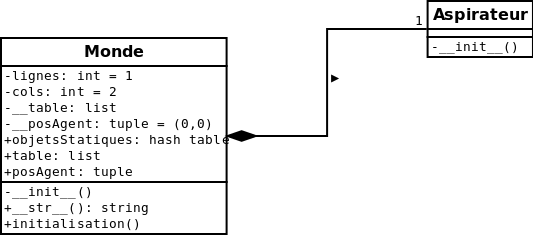
\includegraphics[scale=0.5]{architecture}

\begin{itemize}
 \item \texttt{monde.py} : contient la classe Monde qui contient notre environnement. Nous allons décrire les différents attributs et méthodes:
  \begin{itemize}
  \item \texttt{\_\_init\_\_(aspirateur,lignes,colonnes)} : Constructeur de l'envrironnement;
  \item \texttt{objetsStatiques)} : Renvoie le dictionnaire dont la clé est l'identifiant de l'élément contenu dans le monde. La clé fait référence à un tuple contenant la signification de l'élément et le caractère qu'on lui associe;
  \item \texttt{table} : Renvoie l'état du monde;
  \item \texttt{posAgent} : Renvoie la position de l'aspirateur;
  \item \texttt{\_\_str\_\_} : Affichage du monde (état et aspirateur);
  \item \texttt{initialisation} : Initialise la position de l'aspirateur et l'état du monde de façon stochastique.
  \end{itemize}
 \item \texttt{aspirateur.py} : pass
\end{itemize}

\end{document}
